\begin{table}[H]
\centering
\begin{tabularx}{\linewidth}{@{}>{\centering\arraybackslash}m{3cm}>{\centering\arraybackslash}X>{\centering\arraybackslash}X>{\centering\arraybackslash}X@{}}
\toprule
 & Image 1 & Image 2 & Image 3 \\
\midrule
Pneumoconiosis x-ray & 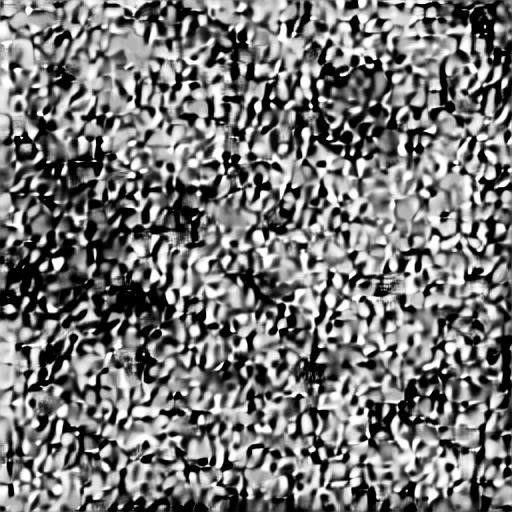
\includegraphics[valign=M,width=\linewidth,height=4cm,keepaspectratio]{main/content/images/sd_hyperdreambooth/pneumoconiosis/xray1.jpeg} & 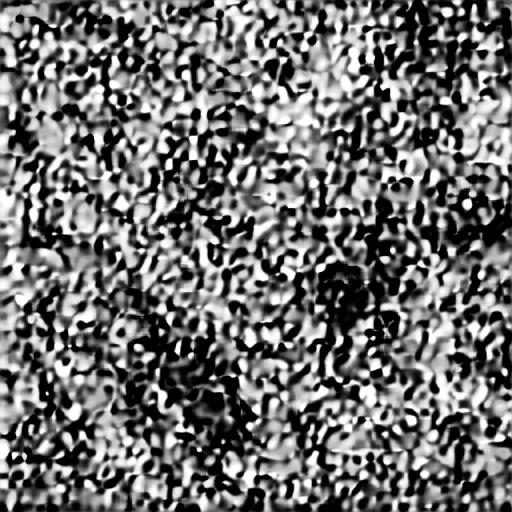
\includegraphics[valign=M,width=\linewidth,height=4cm,keepaspectratio]{main/content/images/sd_hyperdreambooth/pneumoconiosis/xray2.jpeg} & 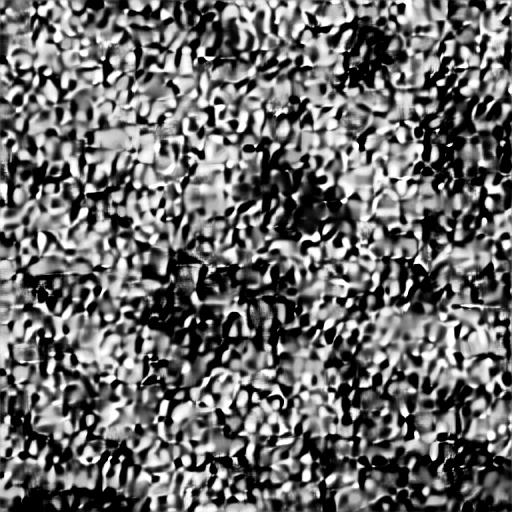
\includegraphics[valign=M,width=\linewidth,height=4cm,keepaspectratio]{main/content/images/sd_hyperdreambooth/pneumoconiosis/xray3.jpeg} \\
\midrule
Human Brain MRI & 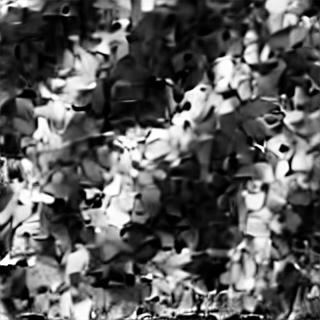
\includegraphics[valign=M,width=\linewidth,height=4cm,keepaspectratio]{main/content/images/sd_hyperdreambooth/brain_tumor/glioma1.jpeg} & 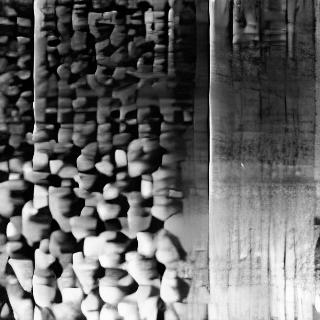
\includegraphics[valign=M,width=\linewidth,height=4cm,keepaspectratio]{main/content/images/sd_hyperdreambooth/brain_tumor/glioma2.jpeg} & 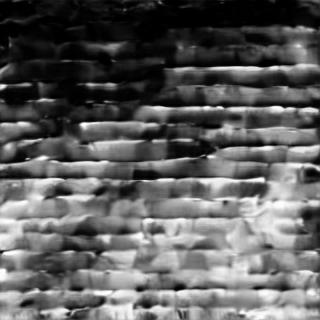
\includegraphics[valign=M,width=\linewidth,height=4cm,keepaspectratio]{main/content/images/sd_hyperdreambooth/brain_tumor/glioma3.jpeg} \\
\midrule
Retinopathy & 
\includegraphics[valign=M,width=\linewidth,height=4cm,keepaspectratio]{main/content/images/sd_hyperdreambooth/retinopathy/hp1.jpeg} & 
\includegraphics[valign=M,width=\linewidth,height=4cm,keepaspectratio]{main/content/images/sd_hyperdreambooth/retinopathy/hp2.jpeg} & 
\includegraphics[valign=M,width=\linewidth,height=4cm,keepaspectratio]{main/content/images/sd_hyperdreambooth/retinopathy/hp3.jpeg} \\
\bottomrule
\end{tabularx}
\caption{Images generated using \textit{HyperDreamBooth} technique with SD v1.5}
\label{tab:image_comparison_hyperdreambooth}
\end{table}
